\section{Classification}

\begin{frame}{The Final Classification (A,B,C,D,E,F,G)}
    % VOCAL CUE: Frase strategica: "By demanding that larger diagrams do not contain loops or hyper-connected nodes (which would violate the Cauchy-Schwarz inequality), the possibilities collapse to:"
    By classifying all "admissible" diagrams (excluding loops and vertices with $>3$ lines to avoid violating Cauchy-Schwarz), we obtain the complete list of simple Lie algebras:

    \begin{itemize}
        \item \textbf{Classical Series:} $A_n (\mathfrak{su}_{n+1})$, $B_n (\mathfrak{so}_{2n+1})$, $C_n (\mathfrak{sp}_{2n})$, $D_n (\mathfrak{so}_{2n})$.
        \item \textbf{Exceptional Algebras:} $G_2, F_4, E_6, E_7, E_8$.
    \end{itemize}

    \begin{figure}
        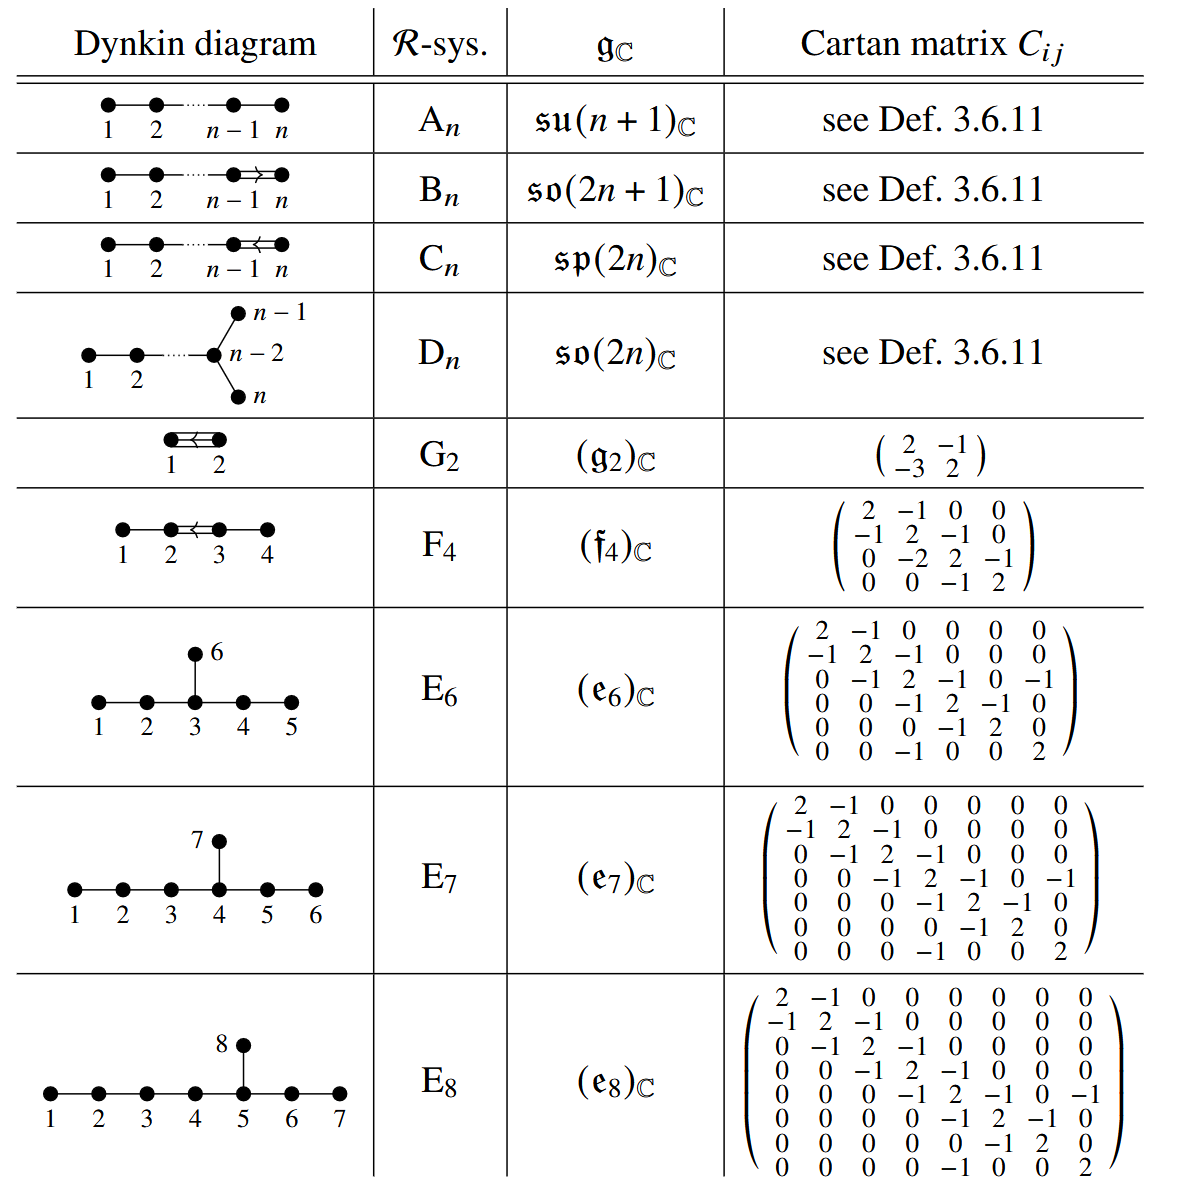
\includegraphics[width=0.9\textwidth]{img/classification-table.png}
    \end{figure}
\end{frame}

\begin{frame}{Accidental Isomorphisms}
    Dynkin diagrams provide an immediate visual proof of "accidental isomorphisms" between seemingly different matrix groups at low rank:

    % VOCAL CUE: Leggi questi isomorfismi. Sono utilissimi in QFT.
    \begin{itemize}
        \item $A_1 \cong B_1 \cong C_1 \iff \mathfrak{su}(2)_\mathbb{C} \cong \mathfrak{so}(3)_\mathbb{C} \cong \mathfrak{sp}(2)_\mathbb{C}$
        \item $B_2 \cong C_2 \iff \mathfrak{so}(5)_\mathbb{C} \cong \mathfrak{sp}(4)_\mathbb{C}$
        \item $A_1 \oplus A_1 \cong D_2 \iff \mathfrak{su}(2)_\mathbb{C} \oplus \mathfrak{su}(2)_\mathbb{C} \cong \mathfrak{so}(4)_\mathbb{C}$
        \item $A_3 \cong D_3 \iff \mathfrak{su}(4)_\mathbb{C} \cong \mathfrak{so}(6)_\mathbb{C}$
    \end{itemize}

    \begin{figure}
        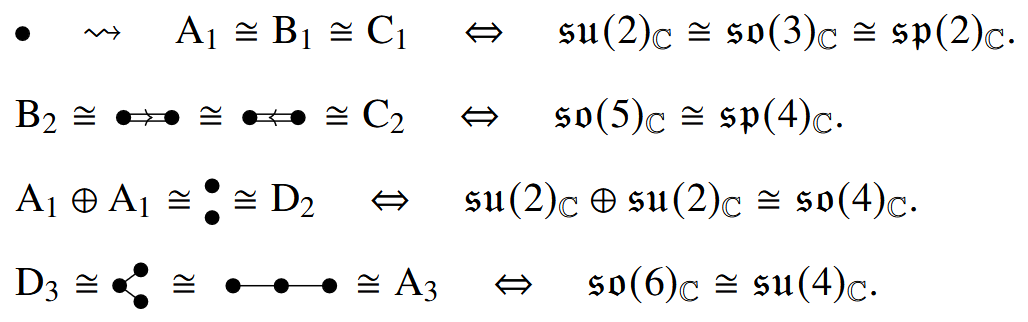
\includegraphics[width=0.6\textwidth]{img/accidental-isomorphisms.png}
    \end{figure}
\end{frame}